\section{Software}

Google Chromecast no es más que un dispositivo compatible con el protocolo propietario Google Cast que actúa como receptor.
Este protocolo fue lanzado en julio de 2013 exclusivo para YouTube, Google Play Music, Google Play Movies \& TV y Netflix, usando como receptor el Chromecast de primera generación. En febrero de 2014 pusieron el SDK a disposición de todos los desarrolladores para usarlo en sus propias aplicaciones.
En mayo de 2015 había más de 20.000 aplicaciones de terceros compatibles con esta tecnología según reconoce Google.

\

Para iniciar la reproducción de un contenido pulsamos el botón de \textit{cast}, que aparecerá automáticamente si Google Cast está integrado con la aplicación.
En ese momento aparecen los dispositivos Chromecast conectados a la red local y se elige aquel donde se quiere emitir el contenido.
Si el receptor es una televisión cuyo HDMI dispone de Consumer Electronics Control (CEC) se encenderá automáticamente.

\

Google Cast tiene dos modos de funcionamiento:

\begin{itemize}

	\item Uno es usar dispositivo desde el que solicitamos el streaming (en adelante dispositivo emisor) para controlar la reproducción: pausar un vídeo, subir el volumen del audio, crear o modificar una cola de reproducción, etc.
	El dispositivo receptor (por ejemplo un Chromecast) es quien se encarga de descargarlo y comunicarse con el servidor de contenido, liberando al dispositivo emisor de esta tarea.
	Esto garantiza una carga de trabajo muy baja para el emisor y le permite estar bloqueado mientras la reproducción está teniendo lugar.
	Ejemplos de aplicaciones que usan este modo de funcionamiento serían Netflix o YouTube.
	Las aplicaciones emisoras de este tipo deben ser compatible con Android 4.1, iOS 7.0 o versiones superiores si son aplicaciones móviles y con Windows 7, macOS 10.7, Chrome OS 28 o versiones superiores si son aplicaciones Chrome.
	En este último caso, se debe tener instalada la extensión Cast.

	\item El otro modo está pensado para enviar contenido del dispositivo emisor, como cuando hacemos mirroring o usamos la televisión como segunda pantalla de una aplicación (por ejemplo en juegos que hacen uso de la Game Manager API).
	El mirroring está soportado de manera nativa en el Chromecast (es decir, no hace falta descargar una aplicación) para pestañas de Chrome, el escritorio de un ordenador con Chrome instalado o dispositivos con Android 4.4 o superior.
	La calidad del streaming en este caso varía ampliamente según la potencia de procesamiento del emisor.
	En el caso de hacerse desde un smartphone, la calidad de las imágenes normalmente se deteriora debido al escalado.

\end{itemize}

\begin{figure*}[h]
	\centering
	\begin{minipage}[b]{.35\textwidth}
		\centering
		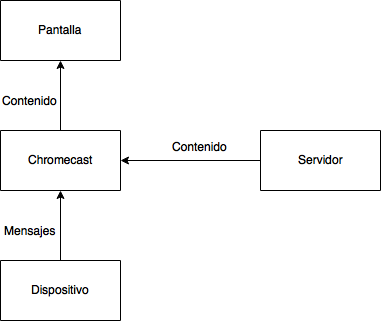
\includegraphics[scale=0.65]{./Imagenes/ChromecastModo1.png}
		\caption{Ilustración del primer modo de funcionamiento de Google Cast}\label{fig:modo1}
	\end{minipage}\qquad
	\hspace{1cm}
	\begin{minipage}[b]{.35\textwidth}
		\centering
		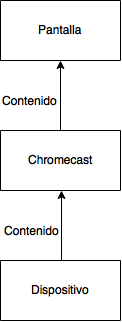
\includegraphics[scale=0.65]{./Imagenes/ChromecastModo2.png}
		\caption{Ilustración del segundo modo de funcionamiento de Google Cast}\label{fig:modo2}
	\end{minipage}
\end{figure*}

Hasta diciembre de 2014, el dispositivo emisor y receptor debían estar conectados a la misma red Wi-Fi para reproducir contenido, pero en las versiones posteriores a esa fecha ya no es necesario.
Esto se debe a que se ha añadido un modo invitado.
En este modo, el receptor emite ultrasonidos a través de los altavoces y el emisor es capaz de localizarlo usando el micrófono.
También puede usarse un PIN de cuatro dígitos que aparece en pantalla.
El modo invitado está disponible para todos los Chromecast con un dispositivo Android como emisor y para los Chromecast a partir de la segunda generación para aquellos con dispositivos iOS como emisor.

\

Como hemos adelantado, la API de Google Cast implementa el paradigma del productor-consumidor. Para implementar el protocolo hacen falta dos aplicaciones:

\begin{itemize}

	\item La aplicación emisora que se encarga de proveer al usuario la capacidad de controlar la reproducción y elegir el dispositivo donde se emite el contenido.
	Esta aplicación crea un canal seguro con la aplicación receptura para el intercambio de mensajes.

	\item La aplicación receptora es una web app ejecutándose en una versión adaptada del navegador Chrome con una interfaz gráfica en CSS.
	Esta puede tener una complejidad muy variable, pudiendo ir desde limitarse a reproducir contenido HTML5 hasta soportar protocolos de streaming como MPEG-DASH, HTTP Live Streaming o el Microsoft Smooth Streaming Protoco\cite{CastSDK}.
	Al ser una web app, el código de la misma debe estar alojado en un servidor, ya que el Chromecast no almacena aplicaciones.
	Una consecuencia de esto último es que, aunque el contenido esté alojado en un dispositivo de la red local, normalmente seguirá siendo imprescindible conexión a internet para cargar la web app. Esto sería posible si la web app también estuviese almacenada en un servidor local, pero es algo que solo tiene sentido para aplicaciones que desarrolle el propio usuario.

\end{itemize}

Los formatos multimedia a los que Google Cast da soporte son los siguientes:

\begin{itemize}

	\item Imágenes en formato BMP, GIF, JPEG, PNG y WEBP, con un límite de 1280x720 píxeles de resolución.

	\item Los codecs de audio HE-AAC, LC-AAC, MP3, Vorbis, WAV (LPCM) y FLAC. AC-3 (Dolby Digital) y E-AC-3 (EC-3, Dolby Digital Plus) están disponibles para passthrough de audio.

	\item Los codecs de vídeo H.264 High Profile Level 4.1 (decodificación hasta 720/60 o 1080/30) y VP8.

\end{itemize}

En el CES de 2015, Google anunció una expansión de Google Cast centrada en la reproducción de audio.
La idea era que los fabricantes de altavoces integraran la tecnología Google Cast sin necesidad de depender de un Chromecast.
Está disponible en varios modelos de LG y Sony.

\

En mayo de 2015, Google lanzó nuevas APIs dirigidas a poder el televisor como segunda pantalla que muestre un contenido distinto del de la aplicación emisora.
Esto, junto con las Game Manager APIs, permite, por ejemplo, usar varios dispostivos como mandos en una partida de un videojuego y una pantalla común que proyecte la partida.
Uno de esos dispositivos sería el que controlara el estado de la partida y se sincronizarían entre ellos intercambiando mensajes con un Chromecast u otro dispositivo receptor.

\begin{figure*}[h]
	\centering
	\begin{minipage}[b]{.35\textwidth}
		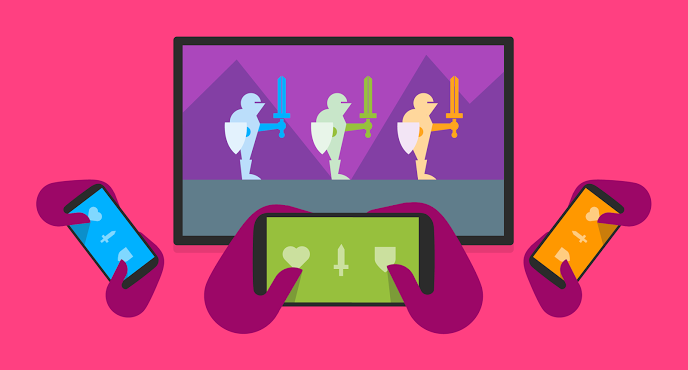
\includegraphics[scale=0.3]{./Imagenes/games.png}
		\caption{Ilustración de Google para explicar el potencial de su Game Manager API}\label{fig:games}
	\end{minipage}\qquad
	\hspace{1cm}
	\begin{minipage}[b]{.35\textwidth}
		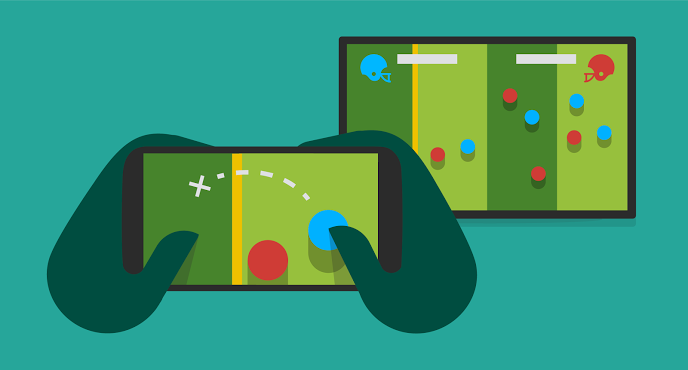
\includegraphics[scale=0.3]{./Imagenes/seconddisplay.png}
		\caption{Ilustración de Google como ejemplo de uso de una pantalla externa a través de Google Cast}\label{fig:seconddisplay}
	\end{minipage}
\end{figure*}

\begin{figure}[h]
	\centering
	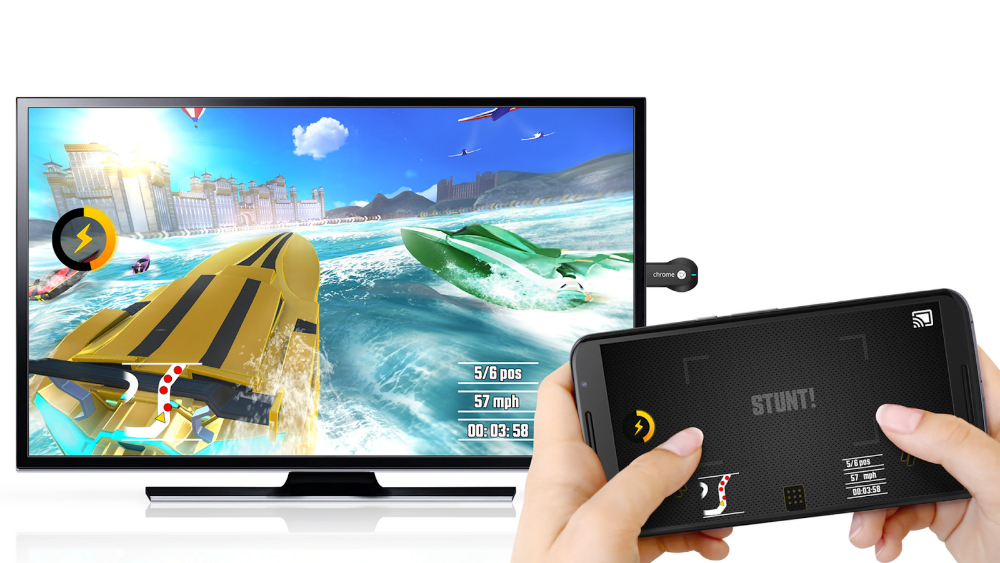
\includegraphics[width=0.6\textwidth]{./Imagenes/gameexample.jpg}
	\label{fig:fondo}
	\caption{Ejemplo de uso de una pantalla externa para videojuegos}
\end{figure}


\subsection{Protocolos que usa Google Cast}

El funcionamiento de Google Cast se descompone en dos pasos: primero, la detección de dispositivos receptores desde la aplicación emisora y, segundo, el intercambio de mensajes entre receptor y emisor.
La primeras versiones del Chromecast usaban el protocolo DIAL para ambos pasos.
En las últimas versiones, para el primer paso se utiliza el protocolo mDNS cuando los dispositivos se encuentran en la misma red local y un protocolo especial basado en ultrasonidos para el modo invitado. Para el segundo paso, Google no ha hecho público qué protocolo se usa. Solo ha trascendido \href{https://plus.google.com/116723992087294619013/posts/d6TLN4S8mrH}{que no usa WebSockets y que se establece un canal binario seguro entre ambos extremos}.

\subsubsection{DIAL}
DIAL (DIscovery And Launch) es el antiguo protocolo de comunicación que usaba Chromecast, desarrollado con Netflix y Youtube.
Se basa en Universal Plug and Play (UPnP), Simple Service Discovery Protocol (SSDP) y protocolos HTTP.
SSDP es un protocolo que sirve para la búsqueda de dispositivos UPnP en una red. Utiliza UDP en unicast o multicast en el puerto 1900 para anunciar los servicios de un dispositivo. Si el receptor ofrece el servicio deseado devuelve el mensaje '200 OK' con HTTP.


\begin{figure}[H]
	\centering
	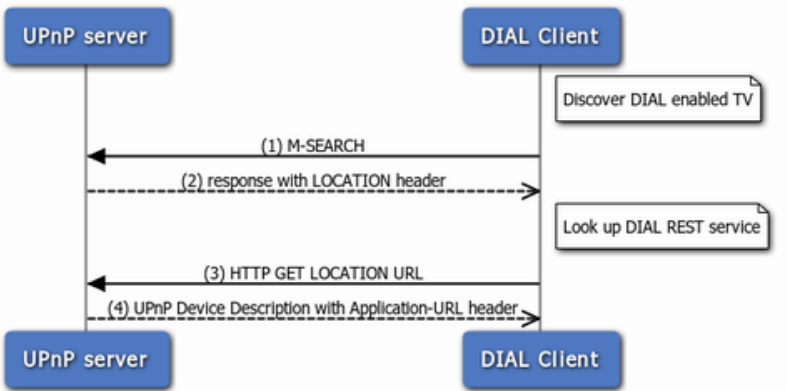
\includegraphics[scale=0.35]{./Imagenes/dial.png}
	\caption{Funcionamiento general DIAL}
	\label{fig:DIAL}
\end{figure}


DIAL permite a dispositivos en segundo plano, como tablets o móviles, enviar contenido a dispositivos en primer plano, por ejemplo televisiones.
Los dispositivos en segundo plano almacenarán el cliente, los de primer plano ejecutarán el servidor.
Para evitar conflictos con los nombres de aplicaciones permitidas DIAL tiene un registro con las aplicaciones que soporta. En el caso de que la aplicación deseada no esté en esa lista puede que tenga un prefijo que esté registrado, para así ofrecer mayor flexibilidad.

\

El protocolo DIAL tiene dos componentes, DIAL Service Discovery y DIAL REST Service.
El primero busca el dispositivo en primer plano dentro de una red local y permite establecer conexión.
El segundo permite al cliente mandar contenido, hacer consultas como subir o bajar volumen, etc. al servidor.
El servidor puede procesar mensajes de hasta 4KB.

\begin{figure}[H]
	\centering
	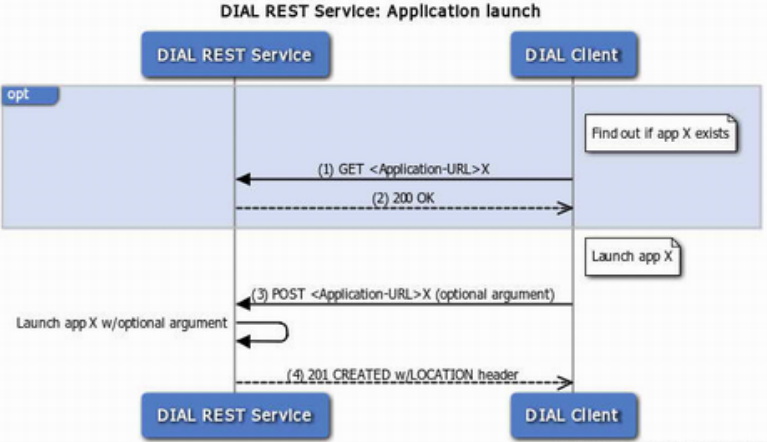
\includegraphics[scale=0.45]{./Imagenes/dialrest.png}
	\caption{Funcionamiento DIAL REST service}
	\label{fig:DIAL}
\end{figure}


Las respuestas específicas y otros detalles como manejo de excepciones se pueden encontrar en \cite{dial}


\subsubsection{mDNS (multicast Domain Name System)}
\begin{figure}[h]
	\centering
	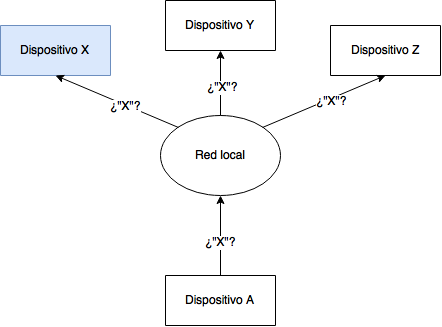
\includegraphics[width=0.6\textwidth]{./Imagenes/mdns1.png}
	\label{fig:mdns1}
	\caption{Primer paso del protocolo mDNS}
\end{figure}

\begin{figure}[h]
	\centering
	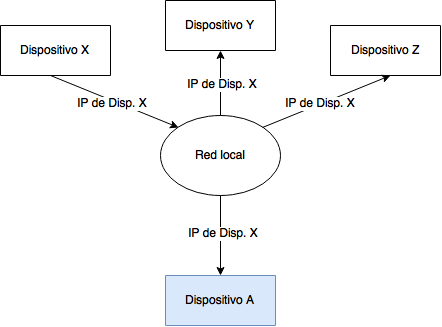
\includegraphics[width=0.6\textwidth]{./Imagenes/mdns2.png}
	\label{fig:mdns2}
	\caption{Segundo paso del protocolo mDNS}
\end{figure}

mDNS es el protocolo usado para encontrar los dispositivos a los que conectarnos.


\subsubsection{Modo invitado vía ultrasonidos}
Si se usa un dispositivo cercano a un Chromecast, este puede detectarlo y sincronizarse vía ultrasonidos.
El Chromecast emite sonidos a muy alta frecuencia (inaudibles para un humano) a través del altavoz de la televisión.
Estos sonidos son la codificación de un mensaje determinado.
A continuación, el emisor escucha este sondo a través del micrófono y lo transforma a un mensaje interpretable por la aplicación.
Este procedimiento está limitado por especificaciones del dispositivos: a menudo, el micrófono no es capaz de detectar sonidos a frecuencias tan altas, bien por limitaciones de hardware o de firmware.
Para entender mejor el funcionamiento del intercambio de información a través de ultrasonidos, se explica con más detalle en \href{http://smus.com/ultrasonic-networking/}{el blog del ingeniero de Google Boris Smus}.

\

Básicamente, hay que establecer un alfabeto de símbolos que se pueden usar en el mensaje, asociando a cada símbolo una frecuencia. Para traducción entre símbolos y sonidos se usa \href{https://en.wikipedia.org/wiki/Dual-tone_multi-frequency_signaling}{DTMF}.

